\subsection[\texorpdfstring{Redes generativas adversariales \\ \textit{Generative Adversarial Networks (GAN)}}{Redes generativas adversariales - Generative Adversarial Networks (GAN)}]%
{Redes generativas adversariales \\ \textit{Generative Adversarial Networks (GAN)}}
% \subsection{Redes generativas adversariales - \textit{Generative Adversarial Networks (GAN)}}

% region Redes generativas adversariales
% TODO: El concepto de redes antagónicas
% TODO: definición matemática de las dos redes
% TODO: Usos y aplicaciones
% TODO: Ventajas e inconvenientes
% TODO: Arquitecturas derivadas
% README: https://arxiv.org/ftp/arxiv/papers/2302/2302.09346.pdf
Las primeras redes neuronales adversariales se presentaron en la década de los 90 como una curiosidad, no fue hasta 2014 con \textit{Ian Goodfellow} que creo y propuso la primera \gls{GAN}. Su arquitectura estaba formada por dos redes neuronales artificiales, una ``generadora (${G}$)'' y otra ``discriminadora (${D}$)''. La red ${G}$ se encarga de generar instancias del mismo dominio que el conjunto de datos, mientras que la red ${D}$ es la encargada de aceptar o rechazar si los datos generados por la red ${G}$ son reales o falsos. Ambas redes se entrenan conjuntamente de manera que ${G}$ minimiza las detecciones de ${D}$, y a su vez ${D}$ detecte las instancias generadas por ${G}$ \cite{de2023redes}.

Las redes generativas pueden contar con lo que se denomina ruido o \textit{latent space}. El \textit{latent space} es una representación abstracta de las características de los datos de entrada que el generador utiliza para crear nuevos ejemplos que se asemejen con las instancias del conjunto de entrenamiento. El objetivo de nuestras redes generadoras es que aprendan a mapear puntos de este espacio latente a puntos del espacio pertenecientes al conjunto de entrenamiento.

\begin{figure}[H]
    \centering
    \centerline{\includesvg[width=0.99\linewidth]{figures/chapter02/GANs-original.drawio.svg}}
    \caption{Arquitectura de las redes neuronales generativas adversariales.\newline{}Fuente: Elaboración propia.}
    \label{fig:gans-architecture}
\end{figure}

% ;TLTR;
Una \gls{GAN} básica se entrena de forma similar a un algoritmo ``${\min\max}$'', esto está representado en la ecuación \ref{eq:gan-0}. Con este proceso hacemos que la red ${G}$ mejore la generación de instancias haciéndola más parecidas, aunque también puede generar instancias irreales, ya que, aunque las instancias sintéticas superan la validación del discriminador, no son físicamente viables en un contexto real.

% TODO: Explicación espacio latente y código latente

Como podemos observar en la ecuación \ref{eq:gan-0} está compuesta por dos secciones similares que luego se suman, estas partes representan las dos redes neuronales compitiendo y la pérdida (\textit{loss}) de ambas, en función de cómo modifiquemos los distintos componentes y estructuras de las redes neuronales la \gls{GAN} se comportara de una forma u otra, estas modificaciones las veremos en las siguientes secciones.
% https://deepgenerativemodels.github.io/assets/slides/cs236_lecture9.pdf
% https://deepgenerativemodels.github.io/notes/gan/

\begin{equation}
    \min_{G}\max_{D} = \mathbb{E}_{x\sim{}P_{\text{data}}(x)} \left[\log\left(D(x\mid{}y)\right)\right] + \mathbb{E}_{z\sim{}P_{\text{noise}}(z)} \left[\log\left(1-D(G(z\mid{}y))\right)\right]
    \label{eq:gan-0}
\end{equation}

Esto está representado en la Figura \ref{fig:gans-architecture}, donde podemos observar las distintas partes de una red \gls{GAN}. Además, podemos observar la distribución de probabilidad aleatoria representada como ${P_{z}, P_{\text{noise}}}$. El objetivo de la red es la optimización de la distribución de probabilidad de la red generativa ${P_{x}, P_{\text{data}}}$ sea similar a ${G(z)}$, es decir, ${G(z)\sim{}P_{g}}$.

\begin{equation}
    \min_{G}\max_{D} = \mathbb{E}_{x\sim{}P_{\text{data}}} \left[\log\left(D(x)\right)\right] + \mathbb{E}_{z\sim{}P_{\text{noise}}(z)} \left[\log\left(1-D(G(z))\right)\right]
    \label{eq:gan-1}
\end{equation}

La función objetiva está definida por la ecuación \ref{eq:gan-2}, nos referimos con ${\theta}$ a los parámetros de la red ${G}$ y con ${\omega}$ a los parámetros de la red ${D}$. La esperanza de ${f(x)}$ con respecto a la distribución de probabilidad de ${x}$ según ${Q}$ es lo que se denota como ${\mathbb{E}_{x \sim Q}}$.

\begin{equation}
    \min_{\theta}\max_{\omega} = \mathbb{E}_{x\sim{}Q} \left[\log\left(D_{\omega}(x)\right)\right] + \mathbb{E}_{z \sim{}P_{\theta}} \left[\log\left(1-D(G_{\theta}(z))\right)\right]
    \label{eq:gan-2}
\end{equation}

Para que la red ${D}$ funcione deberá recibir tantos datos originales ${x_{real}}$ como datos generados por ${G}$, ${x_{fake}}$, ${G}$ se optimiza al mismo tiempo para que ${D}$ no pueda detectar los datos generados por ${G}$, este proceso está representado en las ecuaciones \ref{eq:gan-3-discriminator-loss} y \ref{eq:gan-4-generator-loss}.

% TODO: revisar este texto
Las redes \gls{GAN} originales produce una probabilidad de que la imagen de entrada proceda de la distribución generadora de datos. Usaban una red \textit{feed-fordward} con función final sigmoidea.

En la ecuación \ref{eq:gan-3-discriminator-loss} podemos observar la función de pérdida de la red discriminadora ${(D)}$, la sección ${\log\left(D(x)\right)}$ es la encargada de dar la probabilidad de que está clasificando correctamente la instancia generada por la red ${G}$, maximizando la sección ${\log\left(1 - D(G(z))\right)}$ conseguimos etiquetar correctamente la instancia falsa generada por la red ${G}$.

\begin{equation}
    \nabla_{\omega_{D}} \frac{1}{m} \sum_{i=1}^{m} \left[ \log\left(D(x^{(i)})\right) + \log\left(1-D(G(z^{(i)}))\right) \right]
    \label{eq:gan-3-discriminator-loss}
\end{equation}

En la ecuación \ref{eq:gan-4-generator-loss} podemos observar la función de pérdida de la red generadora ${(G)}$, la pérdida del generador se calcula a partir de la clasificación (Real, Falsa) del discriminador. Se recompensa si consigue engañar al discriminador y se le penaliza en caso contrario.

\begin{equation}
    \nabla_{\theta_{G}} \frac{1}{m} \sum_{i=1}^{m} \log\left(1-D(G(z^{(i)}))\right)
    \label{eq:gan-4-generator-loss}
\end{equation}
% TODO: EXPLICAR Non-Saturating GAN Loss

\subsubsection{Usos y aplicaciones}

Las redes \gls{GAN} se han usado principalmente para la generación de imágenes, aunque puede generar instancias sintéticas de muchos dominios.

% https://paperswithcode.com/method/vae
% https://paperswithcode.com/method/gan
% https://paperswithcode.com/methods/category/convolutions
% https://towardsdatascience.com/paper-explained-high-resolution-image-synthesis-with-latent-diffusion-models-f372f7636d42

% TODO:
% Clasificación de \gls{GAN}
% https://sh-tsang.medium.com/review-lsgan-least-squares-generative-adversarial-networks-gan-bec12167e915
Algunas de las tareas que se pueden realizar con una red \gls{GAN}

\begin{itemize}
    \item \textbf{Síntesis de imágenes:} permite crear una imagen a partir de unos datos de entrada.
    \item \textbf{Imagen a imagen:} permite ``traducir'' una imagen, es decir, transformar una imagen de un estilo a otro.
    \item \textbf{Escalado de imágenes:} aumentar la resolución de una imagen sin perder calidad, generando datos faltantes para no perder detalles.
    \item \textbf{Eliminación de ruido}: limpiar imágenes de baja calidad, son capaces de mejor la claridad y reconstruir artefactos
    \item \textbf{Detección de manipulación de la cámara:} 
    \item \textbf{Codificación de vídeo:} mejorar la eficiencia de compresión de video mediante la generación de cuadros intermedios o reducción de ruido.
\end{itemize}

% \paragraph{Ventajas e inconvenientes}

\subsubsection{Taxonomía de GANs}
% TODO: Referencias para cada uno

% SURVEY:
% https://dl.acm.org/doi/pdf/10.1145/3459992
% https://arxiv.org/ftp/arxiv/papers/2302/2302.09346.pdf
% https://arxiv.org/pdf/2203.11242.pdf                      GANSurvey
% https://www.researchgate.net/publication/349189619_Generative_Adversarial_Networks_in_Computer_Vision_A_Survey_and_Taxonomy

\begin{figure}[H]
    \centering
    \centerline{\includesvg[width=0.99\linewidth]{figures/chapter02/GANs-Taxonomy.drawio.svg}}
    \caption{Taxonomía de GANs.\newline{}Fuente: Elaboración propia, adaptado del artículo ``GANs Survey'' \cite{GANSurvey_2021ZHENGWEIWANG}}
    \label{fig:gan-taxonomy}
\end{figure}


% =============================================================================================================================
\subparagraph{Conditional Generative Adversarial Network (cGAN) [2014]}
% https://towardsdatascience.com/cgan-conditional-generative-adversarial-network-how-to-gain-control-over-gan-outputs-b30620bd0cc8
% https://archive.is/XTMWw
% https://es.mathworks.com/help/deeplearning/ug/train-conditional-generative-adversarial-network.html
% https://github.com/SolClover/Art054_NN_cGAN
% https://arxiv.org/abs/1411.1784       Conditional Generative Adversarial Nets
% https://arxiv.org/abs/2103.14884      Continuous Conditional (cGAN) with Generator Regularization

% https://arxiv.org/abs/2206.13676
% https://arxiv.org/abs/1611.07004
% de la anterior ( sacaron esta: https://arxiv.org/abs/2103.14884

% Pix2Pix
Las redes \gls{cGAN} \cite{cGAN-mirza2014conditional,cGAN-zheng2021continuous,cGAN-li2022ttscgan,cGAN} o GAN condicional fue una de las primeras derivaciones que se crearon, modifica la arquitectura alterando el ruido introducido, permitiendo condicionar la red con información adicional como etiquetas de clase. Esto permite que la red aprenda a generar instancias de una clase dada.

En esta arquitectura se modifica tanto la red generadora ${G}$ como la red discriminadora ${D}$, de forma que ambas deben conocer la clase de la instancia.
% TODO: Hacer gráfico https://datascientest.com/en/wp-content/uploads/sites/9/2023/09/cgan-1.webp
% Hacer gráfico y añadir referencia a pytorch-gan

\begin{equation}
    \min_{G}\max_{D}
    = \mathbb{E}_{x\sim{}P_{\text{data}}(x)}   \left[ \log{\left( D(x\mid{}y)     \right)} \right]
    + \mathbb{E}_{z\sim{}P_{\text{noise}}(z)}  \left[ \log{\left( D(G(z\mid{}y))  \right)} \right]
\end{equation}

\begin{figure}[H]
    \centering
    \centerline{\includesvg[width=0.99\linewidth]{figures/chapter02/GANs-cGAN.drawio.svg}}
    \caption{Arquitectura Conditional GAN (\gls{cGAN})\newline{}Fuente: Elaboración propia.}
    \label{fig:cGAN}
\end{figure}

% =============================================================================================================================
\subparagraph{Deep Convolutional Generative Adversarial Network (DCGAN) [2015]}
% https://paperswithcode.com/method/dcgan
% https://www.tensorflow.org/tutorials/generative/dcgan?hl=es-419
% https://towardsdatascience.com/deep-convolutional-gan-how-to-use-a-dcgan-to-generate-images-in-python-b08afd4d124e
% https://github.com/sthalles/blog-resources/blob/master/dcgan/DCGAN.ipynb
% https://archive.is/MgQCM
% FGSM  -->  https://digibug.ugr.es/handle/10481/72468
Las redes \gls{DCGAN} \cite{DCGAN-radford2016unsupervised,DCGAN-viola2020faultface,DCGAN-aslan2019deep,DCGAN-curto2020highresolution} son una de las redes generativas más famosas y usadas dentro de su ámbito por las ventajas de rendimiento, además estas redes generan detalles de alta resolución partiendo de puntos espacialmente locales de un mapa de características reducido.
% Las GAN convolucionales tradicionales generan detalles de alta resolución en función únicamente de puntos espacialmente locales en mapas de características de menor resolución. 

El discriminador es un clasificador de imágenes basado en \gls{CNN}, frente al generador que a partir de una semilla (ruido) generara imágenes apilando distintas capas.

Las \gls{DCGAN} alteran las capas en ${D}$ cambiando cualquier capa de agrupación (\textit{pooling layers}) por convoluciones escalonadas y en la red ${G}$ las agrupaciones por convoluciones escalonadas fraccionadas, usan \texttt{Batchnorm} en ambas  redes, eliminan capas ocultas de tipo \textit{fully-connected}, usan funciones de activación \texttt{ReLU} en el  generador para todas las capas excepto en la capa de salida que usan \texttt{Tanh} \cite{ibm-gradient-descent}.
% TODO svg

% TODO: ACGAN
% \subparagraph{Auxiliary Classifier Generative Adversarial Network (ACGAN)}






% =============================================================================================================================
\subparagraph{Semi-supervised Generative Adversarial Network (SGAN) [2016]}
% https://towardsdatascience.com/supervised-learning-but-a-lot-better-semi-supervised-learning-a42dff534781
% https://towardsdatascience.com/semi-supervised-learning-with-gans-9f3cb128c5e
% https://archive.is/HCS4V
% https://arxiv.org/abs/1606.01583
En las redes \gls{SGAN} \cite{SGAN-odena2016semisupervised}, la red generadora ${G}$ como la red discriminadora ${D}$ cuentan con datos semi-supervisados, esto difiere de una \gls{GAN} al modificar la red discriminadora con un clasificador. Aprende a clasificar las muestras en diferentes clases en función de las etiquetas dadas.

El uso de estos datos semi-supervisados y de un clasificador en la red discriminadora ${D}$, mejoran los resultados de ambas redes. Además, permite contar con un volumen mayor de datos.

Se ha demostrado que las redes \gls{SGAN} mejoran el rendimiento de la clasificación en conjuntos de datos restringidos.

En la Figura \ref{fig:SGAN} podemos observar la arquitectura de la red usando datos etiquetados, además del clasificador final de la red ${D}$.

\begin{figure}[H]
    \centering
    \centerline{\includesvg[width=0.99\linewidth]{figures/chapter02/GANs-SGAN.drawio.svg}}
    \caption{Arquitectura Semi-supervised GAN ({SGAN})\newline{}Fuente: Elaboración propia.}
    \label{fig:SGAN}
\end{figure}


% \subparagraph{Conditional Generative Adversarial Network (U-Net-GAN)}
% https://arxiv.org/abs/2002.12655
% https://paperswithcode.com/method/u-net-gan
% https://github.com/boschresearch/unetgan
% https://serp.ai/u-net-generative-adversarial-network/

% =============================================================================================================================
\subparagraph{Couple Generative Adversarial Network (CoGAN) [2016]}
% https://medium.com/codex/review-cogan-coupled-generative-adversarial-networks-gan-273f70b340af
% https://github.com/eriklindernoren/PyTorch-GAN/blob/master/implementations/cogan/cogan.py

Las redes \gls{CoGAN} \cite{CoGAN-liu2016coupled} son dos \gls{GAN} que comparten ciertos pesos de las capas, esto permite distribuir de forma conjunta instancias de varios dominios sin necesidad de incluir tuplas.


\begin{equation}
    \begin{split}
        \min_{G_{1},G_{2}}\max_{D_{1},D_{2}}
        & = \mathbb{E}_{x_{1}\sim{}P_{x_{1}}}  \left[ \log{\left( D_{1}(x_{1}) \right)} \right] + \mathbb{E}_{z\sim{}P_{\text{noise}}(z)}      \left[ \log{\left( D_{1}(G_{1}(z))  \right)} \right]   \\
        & + \mathbb{E}_{x_{2}\sim{}P_{x_{2}}}  \left[ \log{\left( D_{2}(x_{2}) \right)} \right] + \mathbb{E}_{z\sim{}P_{\text{noise}}(z)}      \left[ \log{\left( D_{2}(G_{2}(z))  \right)} \right]
    \end{split}
\end{equation}

En la Figura \ref{fig:CoGAN} podemos observar el funcionamiento básico en una iteración de esta arquitectura, lo más relevante es el trabajo  conjunto de ambas redes por sus pesos compartidos, permitiendo que sea un entrenamiento mucho más rápido.

\begin{figure}[H]
    \centering
    \centerline{\includesvg[width=0.99\linewidth]{figures/chapter02/GANs-CoGAN.drawio.svg}}
    \caption{Arquitectura Couple GAN (CoGAN)\newline{}Fuente: Elaboración propia.}
    \label{fig:CoGAN}
\end{figure}


% =============================================================================================================================
% TODO: ContextEncoder

% =============================================================================================================================
\subparagraph{Patch Generative Adversarial Network (PatchGAN) [2016]}

\gls{PatchGAN} \cite{PatchGAN-isola2018imagetoimage} es una arquitectura en la red discriminadora ${D}$, se emplea en tareas de traducción de imagen por ejemplo en redes \gls{Pix2Pix}, la idea principal es simple, segmentar la imagen en parches (${N \times N}$) y discriminar (real o falso) cada uno de esos parches por separado, se centra en analizar las estadísticas de estilo locales y la estructura de alta frecuencia. Estos discriminadores han demostrado que son eficaces a la hora de generar resultados nítidos y de reducir artefactos. Estos discriminadores se suelen usar en conjunto con redes generadoras ${G}$ \gls{U-Net} \cite{U-Net-ronneberger2015unet} para tareas de traducción de imágenes.

A continuación se explica de forma simplificada las ecuaciones de una red \acrshort{PatchGAN}, debemos recordar que estas redes son \acrshort{ConvNET} \href{https://github.com/junyanz/pytorch-CycleGAN-and-pix2pix/issues/39}{PatchGAN Discriminator}

Se ha demostrado que \gls{PatchGAN} reduce los artefactos \cite{PatchGAN-isola2018imagetoimage}, además de que se puede usar en multitud de otras redes como un complemento que mejora la velocidad de entrenamiento y resultados. En el estudio

% Distancia L1
\begin{equation}
    \mathcal{L}_{L1}(G) = \mathbb{E}_{x,y,z} \left[ {\lVert y - G(x,z) \rVert}_{1} \right]
    \label{eq:L1}
\end{equation}

% =============================================================================================================================
\subparagraph{Cycle Generative Adversarial Network (CycleGAN) [2017]}
% https://paperswithcode.com/method/cyclegan
% https://arxiv.org/abs/1703.10593v7
% https://www.tensorflow.org/tutorials/generative/cyclegan?hl=es-419
% https://junyanz.github.io/CycleGAN/
% https://hardikbansal.github.io/CycleGANBlog/
% https://medium.com/analytics-vidhya/the-beauty-of-cyclegan-c51c153493b8
Las redes \gls{CycleGAN} \cite{CycleGAN-zhu2020unpaired,CycleGAN-caleb2021Unpaired,CycleGAN-theiler2019thebeautyofcyclegan} se componen por dos generadores y dos discriminadores, esta red es similar a las redes \gls{Pix2Pix} \cite{pix2pix-isola2018imagetoimage}, ya que lo que hacen es ``traducir'' una instancia a otro dominio, estas redes que a su vez deriva de las redes \gls{cGAN}.

El funcionamiento de estas redes es el siguiente, el primer generador ${\GenXtoY}$, toma la imagen ${x}$ del dominio ${X}$ y la asigna a ${\hat{y}}$, se comprueba con el discriminador ${D_{Y}}$ que ${\hat{y}}$ sea similar a las instancias reales pertenecientes al dominio ${Y}$, este discriminador clasificará si la instancia es una muestra real perteneciente al dominio ${Y}$ o es una instancia generada por ${\GenXtoY}$.

% TODO: terminar explicación de cyclegan

Estas redes permiten extraer las características de un dominio e incorporar esas características a otro dominio con las ventajas de que no necesita de datos de entrenamiento emparejados.

\begin{figure}[H]
    \centering
    \begin{tikzpicture}[node distance=3cm]
        \node (tagX) [draw, minimum size=1.25cm] at (0,0) {$X$};
        \node (tagY) [draw, minimum size=1.25cm, right=of tagX] {$Y$};
        \draw[->, bend left=35] (tagX) to node[above] {${\GenXtoY(x) = \hat{y}}$} (tagY);
        \draw[->, bend left=35] (tagY) to node[below] {${\GenYtoX(y) = \hat{x}}$} (tagX);
        \draw[->, dashed] (tagX.north) -- ++(0,1.25) node[pos=1, right] {$D_{X}$};
        \draw[->, dashed] (tagY.north) -- ++(0,1.25) node[pos=1, right] {$D_{Y}$};
    \end{tikzpicture}
    \caption{Representación CycleGAN}
    \label{fig:fig-cyclegan}
\end{figure}

Función de mapeo para el paso de ${\GenXtoY}$ y el discriminador $D_{Y}$ \ref{eq:cycle-gan-x-to-y}

\begin{equation}
    \begin{split}
        \mathcal{L}_{GAN} (\GenXtoY, D_{Y}, X, Y)
        & = \mathbb{E}_{x\sim{}P_{\text{data}}(x)} \left[\log{\left(1 - D_{Y}(\GenXtoY(x))\right)}\right]     \\
        & + \mathbb{E}_{y\sim{}P_{\text{data}}(y)} \left[\log{\left(D_{Y}(y)\right)}\right]                   \\
    \end{split}
    \label{eq:cycle-gan-x-to-y}
\end{equation}

Función de mapeo para el paso de ${\GenYtoX}$ y el discriminador $D_{X}$ \ref{eq:cycle-gan-y-to-x}

\begin{equation}
    \begin{split}
        \mathcal{L}_{GAN} (\GenYtoX, D_{X}, Y, X)
        & = \mathbb{E}_{x\sim{}P_{\text{data}}(x)} \left[\log{\left(1 - D_{X}(\GenYtoX(x))\right)}    \right]     \\
        & + \mathbb{E}_{y\sim{}P_{\text{data}}(y)} \left[\log{\left(    D_{X}(y)          \right)}    \right]     \\
    \end{split}
    \label{eq:cycle-gan-y-to-x}
\end{equation}

Cada uno de estos generadores ${\GenXtoY}$ y ${\GenYtoX}$ transforman los datos de un dominio a otro, pasando por las siguientes tres fases, \textbf{codificación} usando capas convolucionales, \textbf{transformación} usando bloques \textit{ResNet} y por último la \textbf{descodificación} usando capas convolucionales inversas y una última capa convolucional \cite{CycleGAN-blog}.

A estas dos métricas se le añade la pérdida del ciclo \ref{eq:cycle-gan-l-cyc} esta fórmula se refiere a la consistencia de las transformaciones, si tomamos una instancia del dominio ${X}$ y la pasamos al dominio ${Y}$, si volvemos a pasarla al dominio ${X}$ debe ser consistente.

\begin{equation}
    \begin{split}
        \mathcal{L}_{cyc} (\GenXtoY,\GenYtoX)
        & = \mathbb{E}_{x\sim{}P_{\text{data}}(x)} \left[{\mathrm{MAE}\left(\GenYtoX(\GenXtoY(x)) - x\right)}\right] \\
        & + \mathbb{E}_{y\sim{}P_{\text{data}}(y)} \left[{\mathrm{MAE}\left(\GenXtoY(\GenYtoX(y)) - y\right)}\right] \\
    \end{split}
    \label{eq:cycle-gan-l-cyc}
\end{equation}

En este punto tenemos tres perdidas, a la que podemos añadir la pérdida de la identidad \ref{eq:cycle-gan-l-identity} para mejorar el resultado, esto significa que el generador para datos de un dominio debe dar resultados similares a su dominio, es decir ${\GenXtoY(x) \approx \hat{x}}$ y ${\GenYtoX(y) \approx \hat{y}}$, añadir está pérdida ayuda a preservar las características generales del dominio de origen (colores y tinte en caso imágenes).

\begin{equation}
    \begin{split}
        \mathcal{L}_{identity} (\GenXtoY,\GenYtoX)
        & = \mathbb{E}_{x\sim{}P_{\text{data}}(x)} \left[{\mathrm{MAE}\left(\GenXtoY(x) - x\right)}\right] \\
        & + \mathbb{E}_{y\sim{}P_{\text{data}}(y)} \left[{\mathrm{MAE}\left(\GenYtoX(y) - y\right)}\right] \\
    \end{split}
    \label{eq:cycle-gan-l-identity}
\end{equation}

\begin{itemize}
    \item La pérdida adversarial de ${\GenXtoY}$ contra ${D_{Y}}$.
    \item La pérdida adversarial de ${\GenYtoX}$ contra ${D_{X}}$.
    \item La pérdida del ciclo para el generador ${\GenXtoY}$ y ${\GenYtoX}$.
    \item La pérdida de identidad ${\GenXtoY(x) \approx \hat{x}}$ y ${\GenYtoX(y) \approx \hat{y}}$
\end{itemize}

\begin{equation}
    \begin{split}
        \mathcal{L} (\GenXtoY, \GenYtoX, D_{X}, D_{Y})
        & =            \mathcal{L}_{GAN}       \left(\GenXtoY, D_{Y}, X, Y \right) \\
        & +            \mathcal{L}_{GAN}       \left(\GenYtoX, D_{X}, Y, X \right) \\
        & + \lambda    \mathcal{L}_{cycle}     \left(\GenXtoY,\GenYtoX     \right) \\
        & + 0.5\lambda \mathcal{L}_{identity}  \left(\GenXtoY,\GenYtoX     \right)
    \end{split}
    \label{eq:cycle-gan-all}
\end{equation}

Esta ecuación \ref{eq:cycle-gan-all} es una generalización de cómo funcionan las \gls{CycleGAN}, en cada caso se deberá implementar de forma distinta. En la figura \ref{fig:CycleGAN-2} podemos observar estos dos generadores y los dos discriminadores funcionando para cada uno de los ciclos de entrenamiento.

% \begin{figure}[H]
%     \centering
%     \centerline{\includesvg[width=1\linewidth]{figures/chapter02/GANs-CycleGAN.drawio.svg}}
%     \caption{Arquitectura Cycle GAN (CycleGAN)\newline{}Fuente: Elaboración propia.}
%     \label{fig:CycleGAN}
% \end{figure}

\begin{figure}[H]
    \centering
    \centerline{\includesvg[width=0.99\linewidth]{figures/chapter02/GANs-CycleGAN-2.drawio.svg}}
    \caption{Arquitectura Cycle GAN (CycleGAN)\newline{}Fuente: Elaboración propia.}
    \label{fig:CycleGAN-2}
\end{figure}




% =============================================================================================================================
\subparagraph{Least Square Generative Adversarial Network (LSGAN) [2016]}
% https://paperswithcode.com/method/lsgan
% https://arxiv.org/abs/1611.04076
% https://sh-tsang.medium.com/review-lsgan-least-squares-generative-adversarial-networks-gan-bec12167e915
Las redes \gls{LSGAN} \cite{LSGAN-mao2017squares} o redes generativas de mínimos cuadrados, en estas arquitecturas se modifica la función de pérdida del discriminador, esto mejora la calidad de las instancias generadas así como el proceso de aprendizaje.
% TODO

A continuación en la ecuación \ref{eq:lsgan} se muestra las funciones objetivo para \gls{LSGAN}, debemos tener en cuenta que ${a}$ son los etiquetas para datos falsos, ${b}$ son datos reales y ${c}$ indica el valor que la red ${G}$ envía a la red ${D}$ para que los valide como verdaderos.

\begin{equation}
    \begin{split}
        \min_{D} &= \frac{1}{2} \mathbb{E}_{x\sim{}P_{\text{data}}(x)}  \left[ (D(x) - b)^{2} \right] + \frac{1}{2} \mathbb{E}_{z\sim{}P_{\text{noise}}(z)} \left[ (D(G(z)) - a)^{2} \right]    \\
        \min_{G} &= \frac{1}{2} \mathbb{E}_{z\sim{}P_{\text{noise}}(z)} \left[ (D(G(z)) - c)^{2} \right]                                                                                        \\
    \end{split}
    \label{eq:lsgan}
\end{equation}

En la Figura \ref{subfig:LSGAN-2} podemos observar el límite de decisión de una \gls{GAN} clásica, frente a la Figura \ref{subfig:LSGAN-3} que representa el límite de decisión de una \gls{LSGAN}


\begin{figure}[H]
    \centering
    \captionsetup{justification=centering}
    % 0.99
    \begin{subfigure}{.30\linewidth}
        \centering
        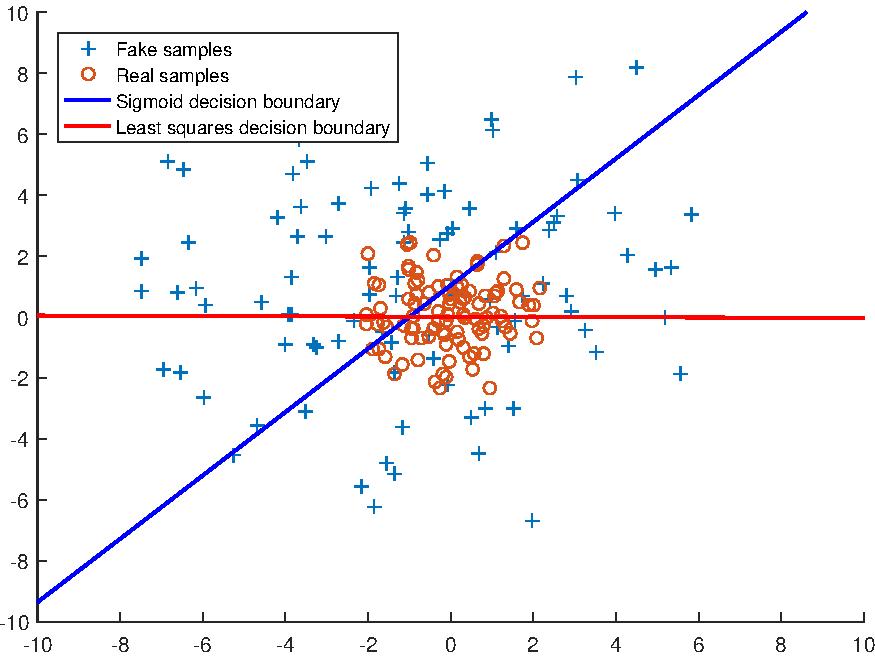
\includegraphics[width=0.95\linewidth]{figures/chapter02/boundary_1.pdf}
        \caption{Límites de decisión de dos funciones de pérdida. }
        \label{subfig:LSGAN-1}
    \end{subfigure}
    \vspace{0.03\linewidth}
    \begin{subfigure}{.30\linewidth}
        \centering
        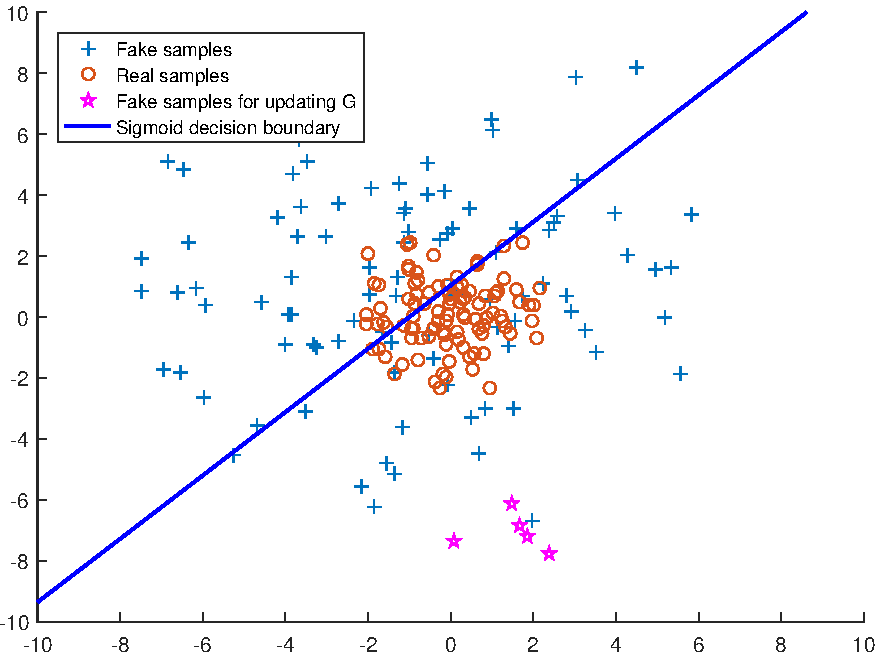
\includegraphics[width=0.95\linewidth]{figures/chapter02/boundary_2.pdf}
        \caption{Límite de decisión de la función de pérdida de entropía cruzada sigmoidea}
        \label{subfig:LSGAN-2}
    \end{subfigure}
    \vspace{0.03\linewidth}
    \begin{subfigure}{.30\linewidth}
        \centering
        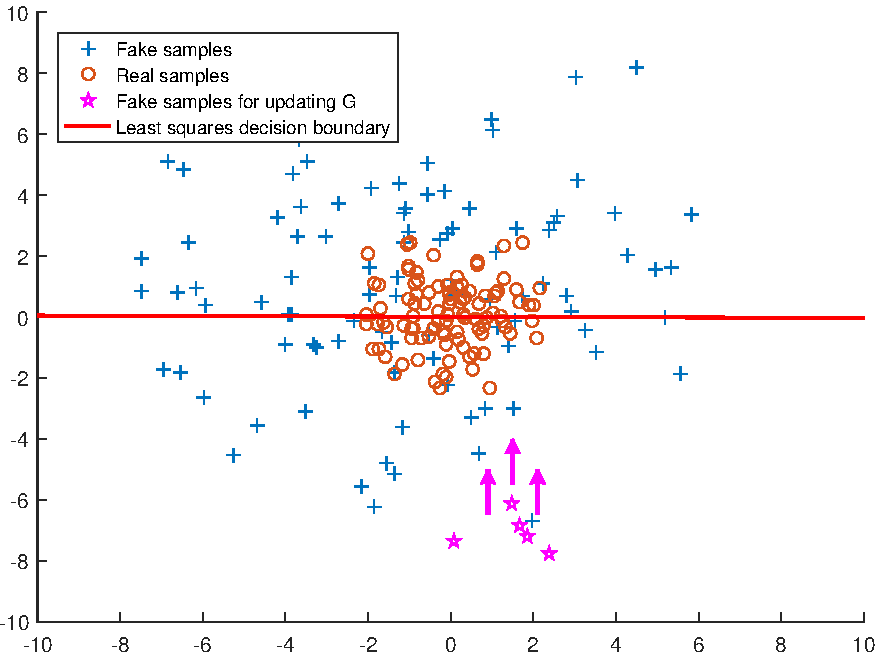
\includegraphics[width=0.95\linewidth]{figures/chapter02/boundary_3.pdf}
        \caption{Límite de decisión de la función de pérdida de mínimos cuadrados.}
        \label{subfig:LSGAN-3}
    \end{subfigure}

    \caption{Least Square Generative Adversarial Network (LSGAN)\newline{}Fuente: Least Squares Generative Adversarial Networks \cite{LSGAN-mao2017squares}}
    \label{fig:LSGAN}
\end{figure}



\subparagraph{Progressive Generative Adversarial Network (ProGAN) [2017]}
% https://paperswithcode.com/method/progan
% https://arxiv.org/abs/1710.10196v3
% https://towardsdatascience.com/explained-a-style-based-generator-architecture-for-gans-generating-and-tuning-realistic-6cb2be0f431

Las redes \gls{ProGAN} o \gls{PGGAN} \cite{ProGAN-karras2018progressive} están basadas en las redes \gls{DCGAN} donde tanto ${G}$ como ${D}$ empiezan con un entrenamiento de imágenes en baja resolución y va aumentando progresivamente la resolución, la idea es hacer que los generadores como los discriminadores vayan aprendiendo progresivamente.

Primero las redes aprenden imágenes de baja resolución ${4 \times 4}$, después ${8 \times 8}$, ${16 \times 16}$, hasta llegar a la resolución, ${1024 \times 1024}$ como vemos en el ejemplo de la Figura \ref{subfig:ProGAN-1}

\begin{figure}[H]
    \centering
    \captionsetup{justification=centering}

    \begin{subfigure}{.475\linewidth}
        \centering
        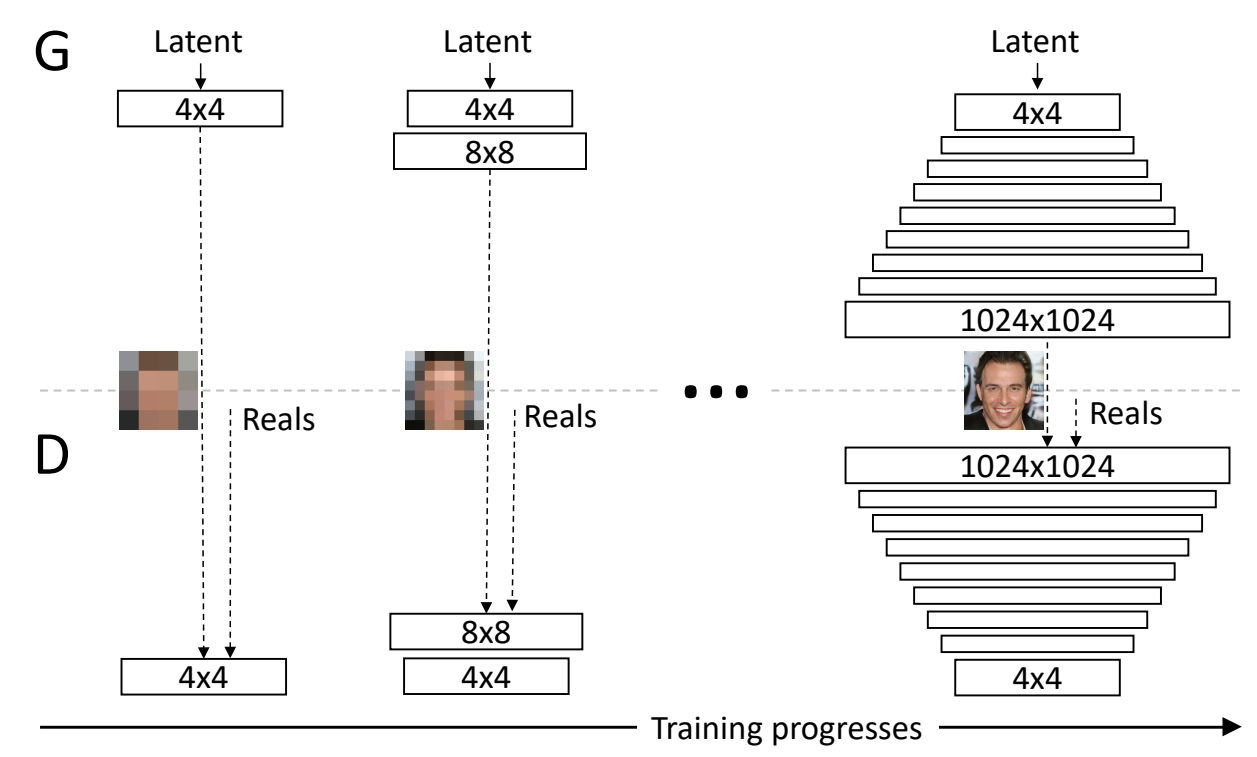
\includegraphics[width=0.75\linewidth]{figures/chapter02/ProGAN-image-32.png}
        \caption{Proceso de entrenamiento de las redes ${G}$ y ${D}$}
        \label{subfig:ProGAN-1}
    \end{subfigure}
    \vspace{0.03\linewidth}
    \begin{subfigure}{.475\linewidth}
        \centering
        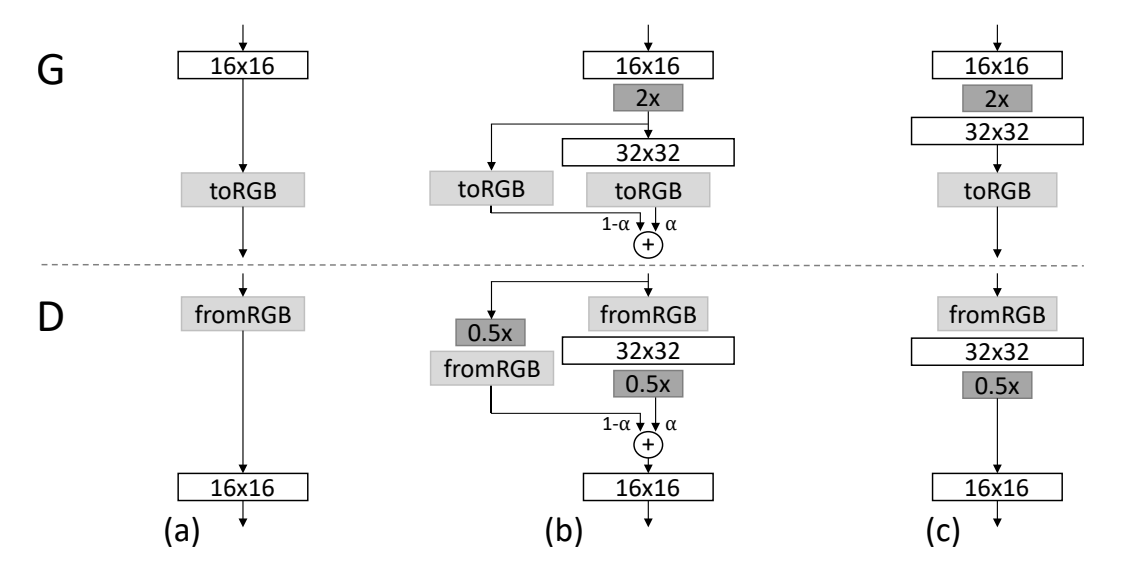
\includegraphics[width=0.75\linewidth]{figures/chapter02/ProGAN-image-16.png}
        \caption{Arquitectura de las redes ${G}$ y ${D}$}
        \label{subfig:ProGAN-2}
    \end{subfigure}

    \caption{Progressive Generative Adversarial Network (ProGAN)\newline{}Fuente: \href{https://blog.paperspace.com/progan/}{ProGAN: Progressive Growing Generative Adversarial Networks}}
    \label{fig:ProGAN}
\end{figure}


\subparagraph{Super Resolution Generative Adversarial Network (SRGAN) [2016]}
% https://paperswithcode.com/method/srgan
% https://arxiv.org/abs/1609.04802
% https://arxiv.org/abs/1711.06491
% https://arxiv.org/abs/1902.06068
% https://homepages.inf.ed.ac.uk/rbf/CVonline/LOCAL_COPIES/VELDHUIZEN/node18.html
Las redes \gls{SRGAN} \cite{SRGAN-ledig2017photorealistic} son una variante de las redes \gls{DCGAN}. Esta red aprende a mapear imágenes de baja resolución a imágenes de alta resolución, utiliza la calidad perceptual en lugar de solo él \gls{PSNR}, estas redes son las que mejores resultados están dando, además de que las abstracciones que aprende no se limitan únicamente al dominio de su entrenamiento sino a la abstracción de formas y patrones en imágenes, estos modelos son sencillos de entrenar y dan buenos resultados.
% TODO

\begin{equation}
    \begin{split}
        \min_{\theta_{G}}\max_{\omega_{D}}~~
        & \mathbb{E}_{I^{H R} {\sim P_{train} (I^{H R})}}  \left[ \log{(D_{\omega_{D}}(I^{H R}))}                      \right]     \\
        & + \mathbb{E}_{I^{L R} {\sim P_{G} (I^{L R})}}    \left[ \log{( 1 - D_{\theta_{D}}(G_{\theta_{G}}(I^{L R})))} \right]     \\
    \end{split}
\end{equation}


\subparagraph{{\small Enhanced Super Resolution Generative Adversarial Network (ESRGAN) [2016]}}
% https://arxiv.org/pdf/1809.00219.pdf
% https://github.com/xinntao/ESRGAN
% https://typeset.io/library/untitled-collection-fu09ijee/esrgan-1809-00219-pdf-3aklgwph
Las redes \gls{ESRGAN} \cite{ESRGAN-wang2018esrgan, SRGAN-ledig2017photorealistic} son una mejora de las \gls{SRGAN}, \gls{ESRGAN} utiliza características antes de la activación para la pérdida perceptual. Esto mejora la consistencia de brillo y la recuperación de texturas. Además, añaden la interpolación de redes para equilibrar la calidad visual y él \gls{PSNR}.

Los investigadores \textit{Xintao Wang, Ke Yu, Shixiang Wu, ...}\cite{ESRGAN-wang2018esrgan} demostraron que las redes \gls{ESRGAN} cuentan con un rendimiento superior a \gls{SRGAN} con un entrenamiento sencillo, contrario a lo que creían los investigadores \textit{Christian Ledig, Lucas Theis, ...} \cite{SRGAN-ledig2017photorealistic} modelos más profundos son más difíciles de entrenar.



\subparagraph{Style Generative Adversarial Network (StyleGAN) [2018]}
% https://paperswithcode.com/method/stylegan
% https://arxiv.org/abs/1812.04948
% https://paperswithcode.com/method/stylegan2
% https://arxiv.org/abs/1912.04958
% Others
% https://arxiv.org/abs/2301.09515

Las redes \gls{StyleGAN} \cite{StyleGAN-karras2019stylebased,StyleGAN-sauer2023stylegant}, es un proyecto desarrollando por NVIDIA, el principal uso de la red es la generación de rostros, actualmente se encuentra en su tercera versión \cite{styleGAN3-karras2021aliasfree}, esta versión cuenta con importantes mejoras de rendimiento, estabilidad, interpolación, entrelazamiento y reducción del \textit{aliasing}. Además, la tercera versión cuenta con la posibilidad de generación de vídeo.

La arquitectura \gls{StyleGAN} \cite{StyleGAN-melnik2023face}, está basada en las redes \gls{PGGAN} que permiten el entrenamiento progresivo, aumentando gradualmente la resolución de las instancias, se introduce la mezcla de estilos de forma distinta a \gls{CycleGAN}, ya que hace un mezclado de los vectores latentes, también añade métodos de inversión con el objetivo de reconstruir vectores latentes de determinadas instancias para manipular editar las instancias en el espacio latente.
% https://towardsdatascience.com/explained-a-style-based-generator-architecture-for-gans-generating-and-tuning-realistic-6cb2be0f431




\subparagraph{Self Attention Generative Adversarial Network (SAGAN) [2018]}
% https://arxiv.org/abs/1805.08318
% https://paperswithcode.com/method/sagan
En las redes \gls{SAGAN} \cite{SAGAN-zhang2018selfattention} permiten modelar dependencias de largo alcance usando técnicas de atención para tareas de generación de imágenes.
Estas redes permiten generar más detalles usando pistas del mapa de características, la red ${D}$ puede comprobar que los rasgos detallados de las instancias generadas son coherentes entre sí.



\subparagraph{Wasserstein Generative Adversarial Network (WGAN) [2017]}
% https://lilianweng.github.io/posts/2017-08-20-gan/
% https://neptune.ai/blog/gan-loss-functions
% https://arxiv.org/abs/1701.07875
% https://paperswithcode.com/method/wgann
% https://medium.com/@mladenkorunoski/wgans-explained-fab61bda2576
Las redes \gls{WGAN} \cite{WGAN-arjovsky2017wasserstein, WGAN-weng2017gan, WGAN-weng2019gan} se basan en la arquitectura clásica de una red \gls{GAN}, pero modifican el discriminador con la intención de que los modelos converjan, esta arquitectura utiliza la distancia de Wasserstein\footnote{La distancia de Wasserstein mide cuánto ``movimiento'' se necesita para transformar una distribución en otra. En términos simples, es como medir la cantidad de trabajo necesario para mover tierra de un lugar a otro.} como función de perdida, esto busca mejorar la estabilidad del entrenamiento y la calidad de las instancias generadas, además evita problemas de colapso de modo\footnote{Durante el entrenamiento, un generador puede ``colapsar'' a una configuración en la que siempre produce las mismas salidas.}.

% Puedes consultar el teorema \ref{theorem::gradW}.

\subparagraph{Wasserstein Generative Adversarial Network with Gradient Penalty (WGAN-GP) [2017]}
% https://neptune.ai/blog/gan-loss-functions
% https://arxiv.org/abs/1701.07875
% https://paperswithcode.com/method/wgan-gp
% https://eva.fing.edu.uy/pluginfile.php/362486/mod_resource/content/3/WGANs.pdf

Las redes \gls{WGAN-GP} \cite{WGAN-GP-gulrajani2017improved} basadas en la arquitectura de las redes \gls{WGAN}, añaden un factor de penalización, mejorando considerablemente la estabilidad del modelo.

Al agregar esta penalización de gradiente, mejora la suavidad en la función de pérdida lo que ayuda a la estabilidad, la penalización, también se recortan los pesos esto ayuda a mantener controlado la continuidad de \textit{Lipschitz} en el discriminador con lo que el modelo converge a una solución más realista.





\subparagraph{Information Maximizing Generative Adversarial Network (InfoGAN) [2016]}
% https://arxiv.org/pdf/1606.03657.pdf
% https://arindam.cs.illinois.edu/courses/f21cs598/slides/gan11_598f21.pdf

% la red generativa ${G}$, se encuentra condicionada de la siguiente forma ${G(z\mid{}c)}$.
Las redes \gls{InfoGAN} \cite{InfoGAN-chen2016infogan}, introduce un discriminador adicional llamado ${Q}$ o red de reconocimiento para controlar las características de las instancias, es la  responsable de estimar los códigos latentes a partir de las instancias generadas. La función objetivo de las redes \gls{InfoGAN} es la regularización de la función objetivo de las \gls{cGAN}. Esto permite controlar la red neuronal de forma que la podamos condicionar a que genere instancias de un dominio y que las instancias generadas contengan ciertas características.

La arquitectura lo logra usando la red ${Q}$ con dos estructuras, una para controlar las variables discretas y otra para las variables continuas del ruido latente, estas variables se utilizan para el cálculo de la perdida. Con esto logra controlar que las instancias generadas sean válidas y coherentes con las clases y características.

\begin{figure}[H]
    \centering
    \centerline{\includesvg[width=0.99\columnwidth]{figures/chapter02/GANs-InfoGAN.drawio.svg}}
    \caption{Arquitectura Information Maximizing GAN (InfoGAN).\newline{}Fuente: Elaboración propia.}
    \label{fig:InfoGAN}
\end{figure}

La arquitectura de \gls{InfoGAN} diferencia entre las redes ${G}$, ${D}$ y ${Q}$, aunque ${D}$ y ${Q}$ comparten la misma arquitectura de red, solo se diferencia en las unidades de salida en la última capa, esto hace que el coste de entrenamiento del modelo sea levemente superior a una red \gls{GAN} clásica, pero con importantes mejoras.

    {\small
        \begin{equation}
            \begin{split}
                \min_{G,Q}\max_{D} V_{InfoGAN}(D,G,Q)   &= V(G,D) - \lambda I(G,Q)      \\
                \min_{G}\max_{D} V_{InfoGAN}(D,G)       &= V(G,D) - \lambda I(c;G(z,c)) \\
            \end{split}
            \label{eq:InfoGAN}
        \end{equation}
    }

${I(c;x)}$ es la información mutua y mide cuanto se sabe de ${c}$ si conocemos ${x}$, es decir si la instancia de $x$ es completamente irrelevante a ${c}$, entonces el discriminador indicara ${I(c;x) = 0}$.

    {\small
        \begin{equation}
            \begin{split}
                I(c; G(z,c))    &=  H(c) - H(c \mid G(z,c))     \\
                &=  H(c) - \mathbb{E}_{x\sim{}G(z,c)}\left[\mathbb{E}_{c'\sim{}P_{c\sim{}x}} \left[ \log{P(c'\mid{}x)}\right]\right]
            \end{split}
        \end{equation}
    }

En el artículo \textit{Interpreting the Latent Space of GANs for Semantic Face Editing} \cite{GANLatentSpace-shen2020interpreting} se propone un método para la interpretación semántica codificada en el espacio latente, esto permite controlar las características de las instancias generadas.



% \subparagraph{Secure Steganography Generative Adversarial Network (SSGAN) [2017]}
% https://arxiv.org/abs/1707.01613
% Las redes \gls{SSGAN} \cite{SSGAN-shi2018ssgan}

% ~V_{SSGAN}(G,D,S)~=~
% \begin{equation}
%     \begin{split}
%         \min_{G}\max_{D}\max_{S}
%         &= \alpha       \left[\mathbb{E}_{x\sim{}P_{\text{data}}(x)} \log(D(x)) + \mathbb{E}_{z\sim{}P_{\text{noise}}(z)} \log(1 - D(G(z)))   \right] \\
%         &+ (1 - \alpha) \left[\mathbb{E}_{z\sim{}P_{\text{noise}}(z)}\log\left( S(\mathrm{Stego}(G(z)))\right)   + \log(1 - S(G(z)))   \right]
%     \end{split}
% \end{equation}


% OTRAS
% https://github.com/jasonshere/FairGAN

\subsubsection{Inversión de GANs}
\label{ch:2:GAN-inversion}
% https://sertiscorp.medium.com/gan-inversion-a-brief-walkthrough-part-i-bc2ee1b73253
% https://sertiscorp.medium.com/gan-inversion-a-brief-walkthrough-part-ii-e192513b89ae
% https://sertiscorp.medium.com/gan-inversion-a-brief-walkthrough-part-iii-da87c28f9e62
% https://sertiscorp.medium.com/gan-inversion-a-brief-walkthrough-part-iv-a72bc713e3c8

Como se especifica en el artículo \cite{GANInversionSurvey-xia2022gan} el generador aprende patrones en el espacio de distribución. Este espacio ${N-\text{dimensional}}$ es el código latente con las características del dominio, se le denomina ${z}$. La inversión de \gls{GAN} proporciona una relación del espacio latente para obtener el código latente del dominio.

El objetivo de la inversión \gls{GAN} es el de obtener el vector latente para cualquier instancia determinada. La obtención de este vector latente proporciona flexibilidad para realizar manipulación de instancias reales en vez de solo poder manipular instancias generadas.

La \gls{GAN} Inversión tiene múltiples aplicaciones, destaca en la manipulación, generación, restauración e interpolación de instancias. Así como en la reconstrucción 3D, comprensión de las instancias, aprendizaje multimodal o imágenes médicas \cite{GANInversionSurvey-xia2022gan}.

\begin{figure}[H]
    \centering
    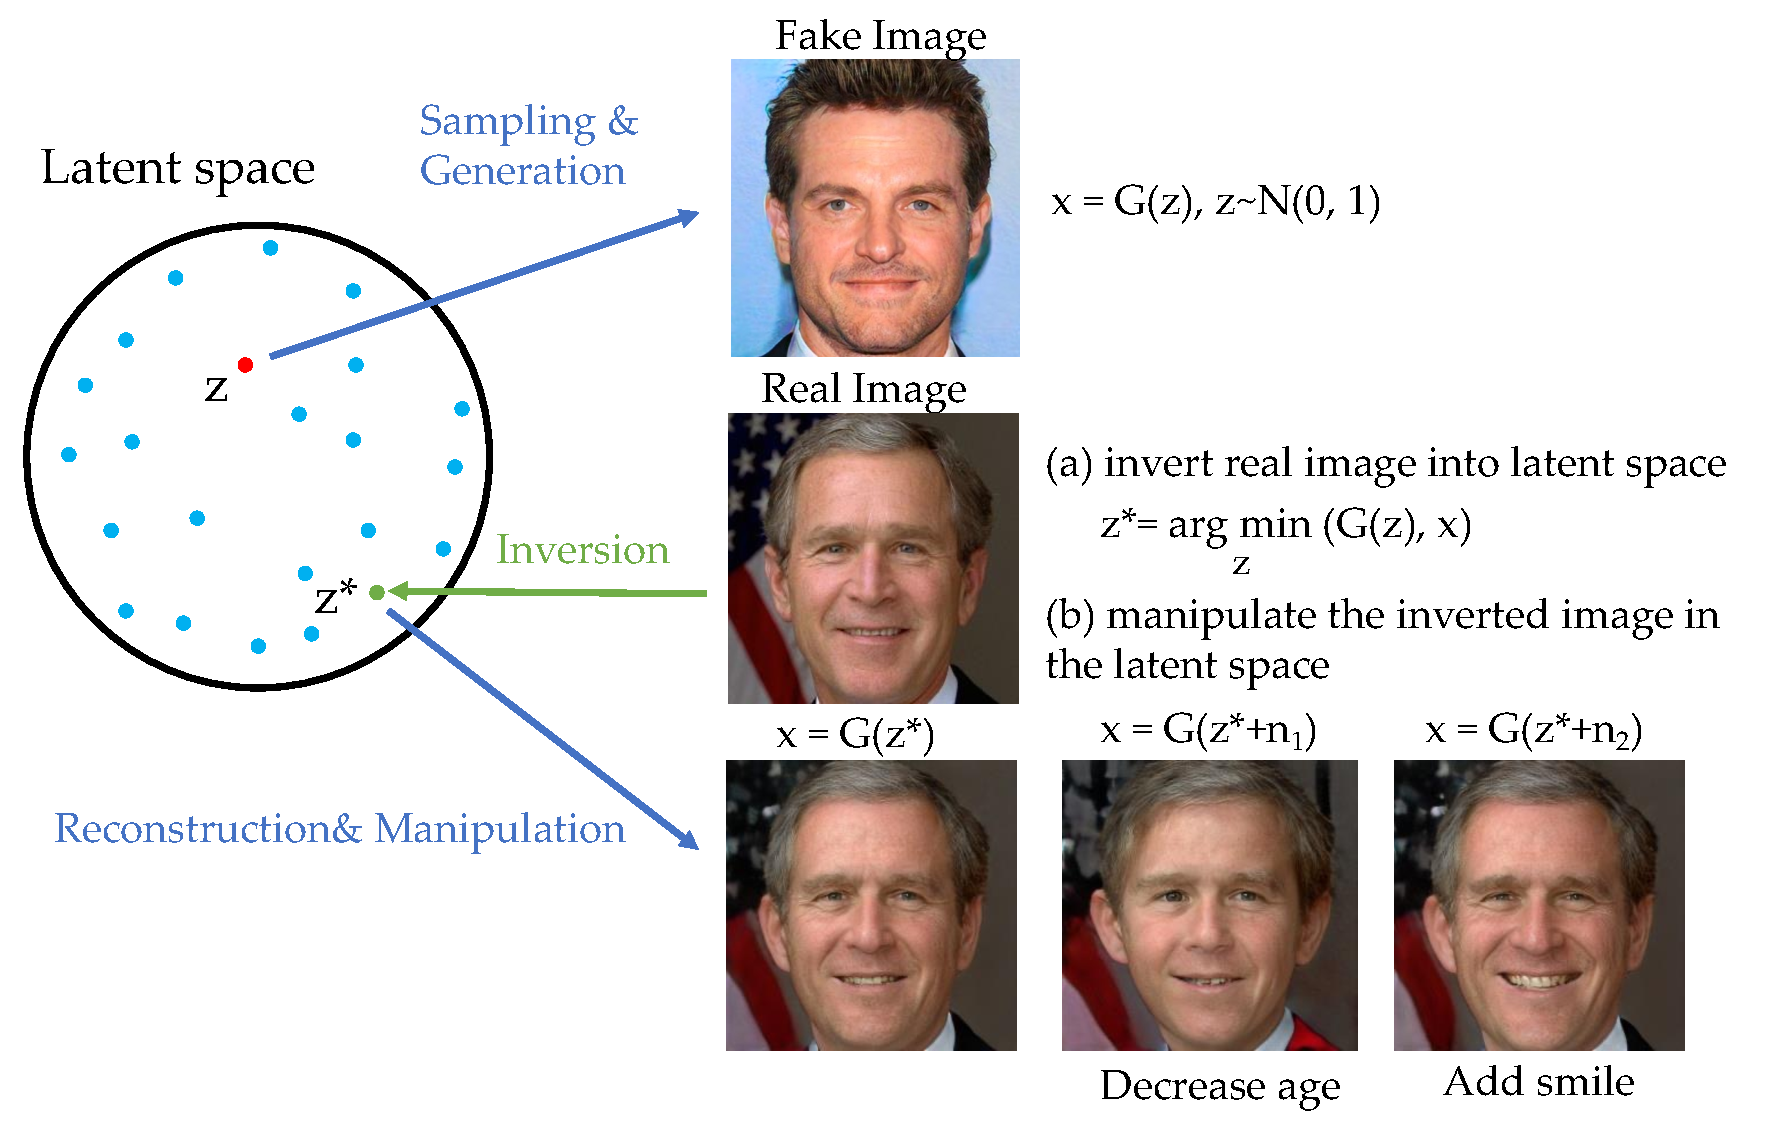
\includegraphics[width=0.5\linewidth]{figures/chapter02/overview.pdf}
    \caption{Ilustración de la inversión de GAN.\newline{}Fuente: GAN Inversion: A Survey \cite{GANInversionSurvey-xia2022gan}}
    \label{fig:gan-inversion}
\end{figure}

Este problema está definido formalmente \ref{eq:inversion-problem-objective-function} como una función objetivo.

\begin{equation}
    z^{*} = \underset{z}{\arg\min}\, \ell\left( G(z), x \right),
    \label{eq:inversion-problem-objective-function}
\end{equation}

A continuación, en la Figura \ref{fig:gan-inversion-methods} se presentan el flujo para la extracción del vector del código latente de los distintos métodos que han propuesto en el artículo \cite{GANInversionSurvey-xia2022gan}.

\begin{figure}[H]
    \centering
    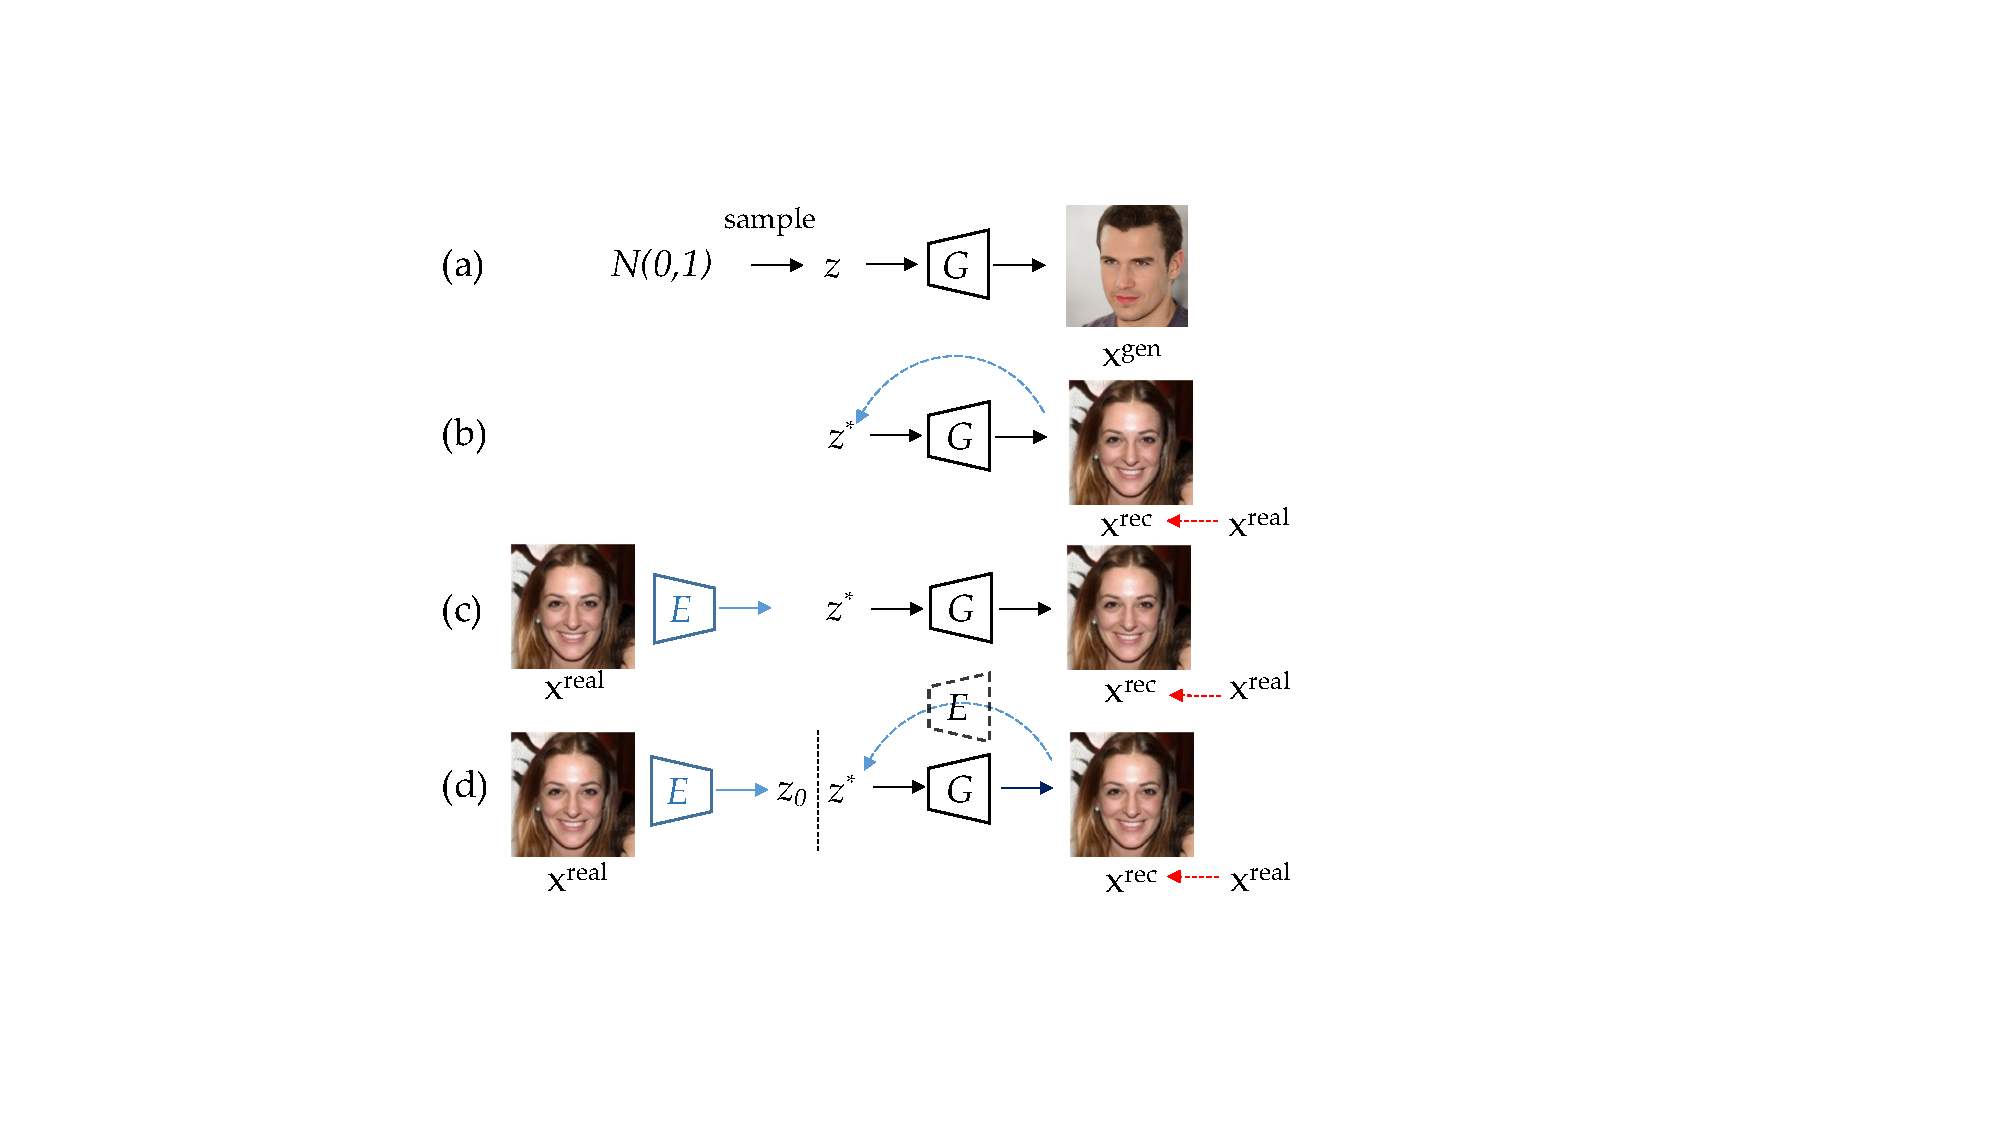
\includegraphics[width=0.5\linewidth]{figures/chapter02/inversion_types.pdf}
    \caption{Tipos de GAN inversión.\newline{}Fuente: GAN Inversion: A Survey \cite{GANInversionSurvey-xia2022gan}}
    \label{fig:gan-inversion-methods}
\end{figure}

En la sección \textbf{a} de la Figura \ref{fig:gan-inversion-methods} podemos observar una \gls{GAN} clásica sin ningún método de inversión.

En la sección \textbf{b} de la Figura \ref{fig:gan-inversion-methods} podemos ya ver el método \textit{Optimization-based} optimiza el vector latente ${z}$ para reconstruir una imagen ${x^{\text{rec}}}$ cercana a la instancia real ${x}$. La función objetivo es la definida en la ecuación \ref{eq:GAN-inversion--optimization-based}.

\begin{equation}
    z^{*} = \underset{z}{\arg\min}\, \ell(x, G(z; \theta))
    \label{eq:GAN-inversion--optimization-based}
\end{equation}

En la sección \textbf{c} de la Figura \ref{fig:gan-inversion-methods} podemos observar el método \textit{Learning-based} que incorpora un módulo codificador llamado ${E}$ que se entrena utilizando instancias generadas por ${G}$ con sus vectores latentes. Es decir, el codificador ${E}$ intenta generar un vector latente denominado ${z_{n}}$ para la instancia ${x_{n}}$ tal que cuando el vector latente se pase a la red ${G}$. La función objetivo es la definida en la ecuación \ref{eq:GAN-inversion--learning-based}.

\begin{equation}
    {\theta}_{E}^{*} = \underset{\theta_{E}}{\arg\min} \sum_{n}{ \mathcal{L}(G(E(x_{n};\theta_{E})),x_{n})  }
    \label{eq:GAN-inversion--learning-based}
\end{equation}

En la sección \textbf{d} de la Figura \ref{fig:gan-inversion-methods} podemos observar el método \textit{Hybrid-based} que incorpora los enfoques \textit{Optimization} y \textit{Learning}. Durante la inferencia, la instancia real ${x}$ se pasa al codificador ${E}$ con el que se obtiene ${z}$, este valor será la inicialización ${z_{0}}$ del vector latente de optimización para reducir la distancia entre la instancia real ${x}$ y la instancia reconstruida ${x^{\text{rec}}}$

\subparagraph{Aplicaciones de la inversión de GANs}

Algunos investigadores han estudiado la inversión de GANs para diseccionar GANs y comprender sus abstracciones internas, esto también sirve para entender qué características las GANs no aprenden.

\textbf{Interpolación de instancias}:
Una posibilidad es usar una interpolación lineal en el espacio latente, con ello podemos fusionar dos vectores latentes en el espacio latente, esto logra una transición suave

\begin{equation}
    \mathrm{z} = \mathrm{z}_{1}(\lambda) + \mathrm{z}_{2}(1 - \lambda) ~\text{donde}~ \lambda \in (0,1)
\end{equation}

Nos referimos como ${\mathrm{z}}$ al vector latente de la interpolación de las dos instancias ${\mathrm{z}_{1}}$ y ${\mathrm{z}_{2}}$ y ${\alpha}$ es el factor de paso

\textbf{Manipulación de instancias}:
Mediante una transformación lineal en el espacio latente, se puede lograr una manipulación de las instancias, esto se logra transformando el código latente de la imagen en direcciones semánticas específicas.

\begin{equation}
    \begin{split}
        \mathrm{x}^{\prime} &= G(\mathrm{z}^{\prime}) \\
        \mathrm{z}^{\prime} &= \mathrm{z} + \alpha ~n
    \end{split}
\end{equation}

Nos referimos como ${\mathrm{z}^{\prime}}$ y ${\mathrm{x}^{\prime}}$ al código latente manipulado de la instancia, ${\alpha}$ es el factor de paso y ${n}$ es la dirección semántica específica del espacio latente.

\textbf{Difusión semántica}:
De forma similar a \textit{Context Encoder} se hace un recorte de la instancia para fusionar junto con otra instancia recortada y difuminar la fusión de ambas instancias, el objetivo es que la instancia generada conserve las características de la imagen destino.

\begin{figure}[H]
    \captionsetup[subfigure]{justification=centering}
    \begin{subfigure}{.60\linewidth}
        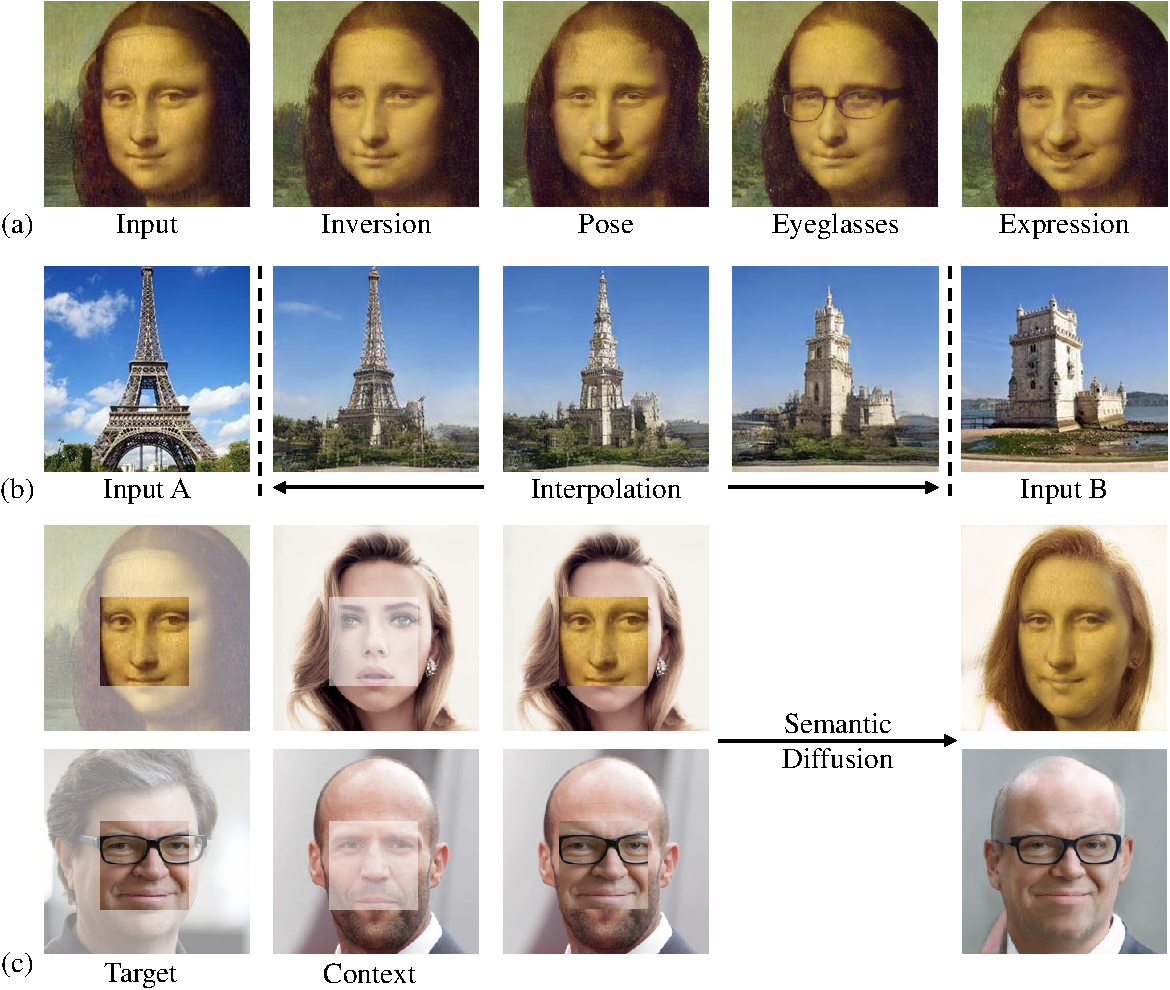
\includegraphics[width=\linewidth]{figures/chapter02/main_teaser.pdf}
        \caption{Difusión semántica}
        \label{subfig:semantic-diffusion}
    \end{subfigure} 
    \hfill
    \begin{subfigure}{.35\linewidth}
        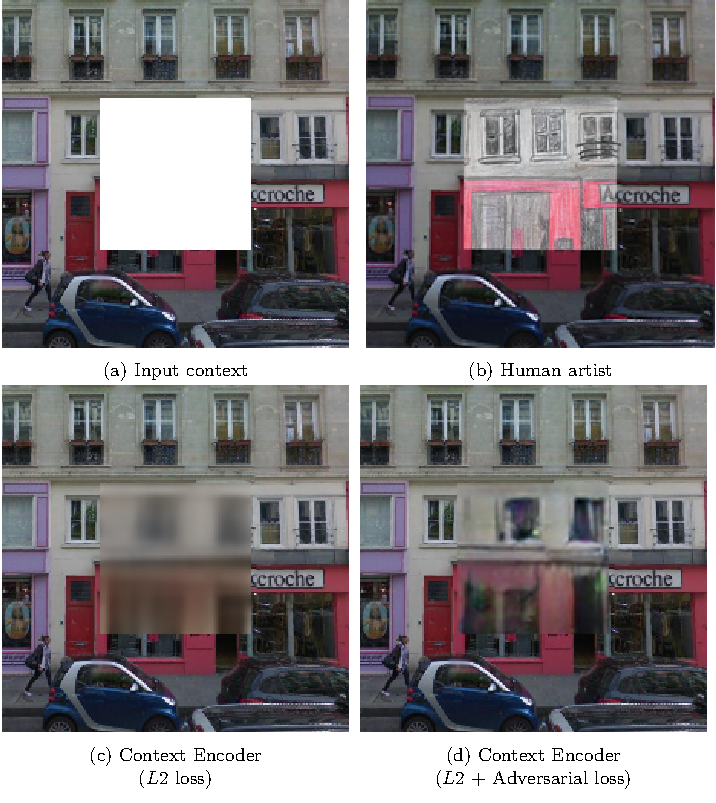
\includegraphics[width=\linewidth]{figures/chapter02/context-encoder.pdf}
        \caption{Context Encoder}
        \label{subfig:context-encoder}
    \end{subfigure}

    \caption{Diferencias entre Difusión semántica y Context Encoder}
    \label{fig:context-encoder-vs-semantic-diffuson}
\end{figure}



% endregion Redes generativas adversariales
